\documentclass[12pt,twoside]{article}
\usepackage{light}
\usepackage{subfigure}
\usepackage{graphicx}
\newcommand{\proofrubric}[3][Any correct proof.]
  {
  	\begin{center}
	\fbox{\begin{minipage}{35em}
	\textbf{Rubric}
	\par
	[#3pts] #1
		\begin{center}
		\textbf{or}
		\end{center}
	#2
	\end{minipage}}
	\end{center}
  }
  
  \newcommand{\rubric}[1]
  {
  	\begin{center}
	\fbox{\begin{minipage}{35em}
	\textbf{Rubric}
	\par
	#1
	\end{minipage}}
	\end{center}
  }
\hidesolutions
\showsolutions

\newcommand{\TAonename}{Henry}
\newcommand{\TAtwoname}{Emanuele}
\newcommand{\TAthreename}{Rachel}
\newcommand{\TAfourname}{Patrick}
\newcommand{\TAfivename}{Devin}
\newcommand{\TAsixname}{Tally}
\newcommand{\TAsevenname}{Michael}
\newcommand{\TAeightname}{Wei-En}
\newcommand{\TAninename}{Sean}


\begin{document}

\problemset{4}{September 27, 2016}{Monday, October 3}
\noindent \textbf{Reading Assignment:}   Sections 4.5.1, 4.6.4, 4.8, 5.0, 5.1, 5.3
\\

\begin{problem}{15}
Euler's theorem states that for any integer $n$, if $a$ is \textbf{relatively prime} to $n$, then $a^{\phi(n)} \equiv 1$ (mod $n$), where $\phi(n)$ is referred to as the Euler totient function ($\phi(n)$ is also equal to the number of positive integers less than $n$ that are relatively prime to $n$).  In particular, if $n = pq$ for primes $p, q$, then $\phi(n) = (p-1)(q-1)$.   
\bparts
\ppart{10}  In RSA, we used an application of Euler's theorem to essentially ``conclude'' that $m^{ed} \equiv  m$ (mod $pq$) for integers $e, d$ such that $ed \equiv 1$ (mod $(p-1)(q-1)$). But what happens if $m = p$ or $m = q$?  Clearly, we have that $p$ and $q$ are not relatively prime to $pq$.  Nevertheless, show that if $m = p$ or $m = q$, we still have that $m^{ed} \equiv m$ (mod $pq$).
\proofrubric{
[5pts] $p^{1+k(p-1)(q-1)} \equiv p \pmod {pq}$ or $pq \mid p^{1+k(p-1)(q-1)} - p$ ($1+k(p-1)(q-1)$ can be replaced by $ed$ \par
[5pts] $q \mid p^{k(p-1)(q-1)} - 1$ by Fermat's little theorem.
}{10}
\solution{
We will show that the statement holds for $m = p$.  Then by symmetry, we can conclude that the statement holds for $m = q$.  First, if $ed \equiv 1$ (mod $(p-1)(q-1)$), then there exists some integer $k$ such that $ed = 1 + k(p-1)(q-1)$ by definition.  Hence we must show that $p^{1+k(p-1)(q-1)} \equiv p \pmod {pq}$.  But this is equivalent to showing that $pq \mid p^{1+k(p-1)(q-1)} - p$.

Now $ p^{1+k(p-1)(q-1)} - p = p(p^{k(p-1)(q-1)} - 1)$.  Hence we just need to show that $q \mid p^{k(p-1)(q-1)} - 1$.  But this is true by Fermat's little theorem as $p,q$ are relatively prime.  
}

\ppart{5} Suppose Alice and Bob are communicating using RSA.  Alice generates a pair of primes, and computes $N_A$, which is the product of those primes.  Similarly, Bob generates a pair of primes, and computes $N_B$, which is the product of those primes.  Unfortunately, one of the primes Bob uses to construct $N_B$ is the same as one of those Alice used to construct $N_A$.  How can a third party Eve now eavesdrop on communications between Alice and Bob if $N_A \neq N_B$?
\rubric{
[2pts] gcd of $(N_A, N_B)$ will be prime $p$.\par
[2pts] $\frac{N_A}{p}, \frac{N_B}{p}$ gives the other primes. \par
[1pt] Use Pulverizer to find $d$.
}

\solution{
First Eve calculates the gcd of $(N_A, N_B)$, which must be the common prime $p$ used by both Bob and Alice since $N_A \neq N_B$ and each of $N_A, N_B$ is a product of exactly two primes.  Hence Eve can then compute $\frac{N_A}{p}, \frac{N_B}{p}$ to find the primes that Alice and Bob are using.  Now, given Alice and Bob's public keys, Eve can then use the Pulverizer to compute their private keys.  Hence, Eve is then able to completely unravel the RSA scheme used by Alice and Bob.
}
\eparts
\end{problem}

\begin{problem}{15} In this problem, we will investigate systems of linear congruence equations. 
\bparts

\ppart{5} Find the smallest positive integer $x$, which leaves a remainder $1$ when divided by $3$ and leaves a remainder $3$ when divided by $7$. (\textit{Hint}: If $x$ leaves a remainder $1$ when divided by $3$, write $x = 1 + 3k_1$ for some integer $k_1$, and consider $1 + 3k_1 \equiv 3$ (mod $7$))
\rubric{
[-1pt] Math errors.\par
[5pts] $x = 10$.
}
\solution{
As suggested in the hint, we let $x = 1 + 3k_1$.  Then we consider 
\begin{equation*}
\begin{split}
1 + 3k_1 &\equiv 3 \pmod 7 \\
3k_1 &\equiv 2 \pmod 7 \\
k_1 &\equiv 10 \pmod 7 ~~ \text{Since we have that the inverse of 3 mod 7 is 5}\\
\end{split}
\end{equation*}

Now by definition, there must be some integer $k_2$ for which $k_1 = 10 + 7k_2$.  Substituting back into the equation for $x$, we conclude that $x = 1 + 3(10 + 7k_2) = 31 + 21k_2$.  Hence we substitute $k_2 = -1$ to find the smallest positive integer $x = 10$.  
}

\ppart{10} For integers $a$ and $b$ and for relatively prime integers $m, n$, find a range of solutions to
\begin{align*}
    x &\equiv a \pmod{m} \\
    x &\equiv b \pmod{n} \\
\end{align*}
\rubric{
[-1pt] Math errors. \par
[6pts] Follow the same steps as taken in part (a).\par
[4pts] $x = a + (s(b-a) + nk_2)m$ or $a + s(b-a)m + nmk_2$.
}
\solution{
We follow the same procedure outlined in the part above.  Since $x \equiv a \pmod m$, let $x = a + k_1m$ for some integer $k_1$.  Then substitute this equation into $x \equiv b \pmod n$:
\begin{equation*}
\begin{split}
a + mk_1 &\equiv b \pmod n \\
mk_1 &\equiv b-a \pmod n \\
k_1 &\equiv s(b-a) \pmod n ~~ \text{Where s is the inverse of m mod n }\\
\end{split}
\end{equation*}

Now by definition, there must be some integer $k_2$ for which $k_1 = s(b-a) + nk_2$.  Substituting back into the equation for $x$, we conclude that:

 $x = a + (s(b-a) + nk_2)m = a + s(b-a)m + nmk_2$
 
is a range of solutions to the system of congruences.

}
\eparts
\end{problem}



\begin{problem}{15}
Recall that a \term{coloring} of a simple graph is an assignment of a color
to each vertex such that no two adjacent vertices have the same color.  A
\term{$k$-coloring} is a coloring that uses at most $k$ colors.

\begin{falseclm*}
Let $G$ be a (simple) graph with maximum degree at most $k$.  If $G$ also
has a vertex of degree less than $k$, then $G$ is $k$-colorable.
\end{falseclm*}

\bparts \ppart{5}\label{counterexample} Give a counterexample to the False
Claim when $k=2$. 
\proofrubric[Any correct counterexample]{
[5pts] One node by itself, and a separate triangle.
}{5}
\solution{One node by itself, and a separate triangle
($K_3$).  The graph has max degree 2, and a node of degree zero, but is not
2-colorable.}

\ppart{10} Consider the following proof of the False Claim:

\begin{proof}

Proof by induction on the number $n$ of vertices:

{\bf Induction hypothesis:}
$P(n)$ is defined to be:  Let $G$ be a graph with $n$ vertices and maximum degree at most $k$.  If $G$ also has a vertex of degree less than $k$, then $G$ is $k$-colorable.

{\bf Base case:} (n=1) $G$ has only one vertex and so is 1-colorable.  So
$P(1)$ holds.

{\bf Inductive step:}

We may assume $P(n)$.  To prove $P(n+1)$, let $G_{n+1}$ be a graph with
$n+1$ vertices and maximum degree at most $k$.  Also, suppose $G_{n+1}$
has a vertex, $v$, of degree less than $k$.  We need only prove that
$G_{n+1}$ is $k$-colorable.

To do this, first remove the vertex $v$ to produce a graph, $G_n$, with
$n$ vertices.  Removing $v$ reduces the degree of all vertices adjacent to
$v$ by 1.  So in $G_n$, each of these vertices has degree less than $k$.
Also the maximum degree of $G_n$ remains at most $k$.  So $G_n$ satisfies
the conditions of the induction hypothesis $P(n)$.  We conclude that $G_n$
is $k$-colorable.

Now a $k$-coloring of $G_n$ gives a coloring of all the vertices of
$G_{n+1}$, except for $v$.  Since $v$ has degree less than $k$, there will
be fewer than $k$ colors assigned to the nodes adjacent to $v$.  So among
the $k$ possible colors, there will be a color not used to color these
adjacent nodes, and this color can be assigned to $v$ to form a
$k$-coloring of $G_{n+1}$.
\end{proof}

Identify the exact sentence where the proof goes wrong.\\
\rubric{
[10pts] Correct sentence with correct reasoning.\par
\begin{center}
\textbf{or}
\end{center}
[5pts] Correct reasoning of ``if $v$ has degree 0,
  then removing $v$ will not reduce the degree of any vertex, and so there
  may not be any vertex of degree less than $k$ in $G_n$"\par
\begin{center}
\textbf{and one of} \par
\end{center}
[3pts] Removing $v$ reduces the degree of all vertices adjacent to
$v$ by 1. \par
[5pts] So in $G_n$, each of these vertices has degree less than $k$.
}
\solution{``So $G_n$ satisfies the conditions of the
  induction hypothesis $P(n)$.''  The flaw is that if $v$ has degree 0,
  then removing $v$ will not reduce the degree of any vertex, and so there
  may not be any vertex of degree less than $k$ in $G_n$, as in the
  counterexample of part~\eqref{counterexample}."}


\eparts
\end{problem}

\begin{problem}{15}
Two graphs are isomorphic if they are the same up to a relabeling of their vertices (see Definition 5.1.3 in the
 book). A property of a graph is said to be \emph{preserved under isomorphism} if
whenever $G$ has that property, every graph isomorphic to $G$ also has
that property.  For example, the property of having five vertices is
preserved under isomorphism: if $G$ has five vertices then every graph
isomorphic to $G$ also has five vertices.

\bparts
\ppart{5}
Some properties of a simple graph, $G$, are described below. Which of these properties is {\em preserved under isomorphism}?

\begin{enumerate}
\item
$G$ has an odd number of vertices.

\item
None of the labels of the vertices of $G$ is an even integer.

\item
$G$ has a vertex of degree 3.

\item
$G$ has a exactly one vertex of degree 3.

\end{enumerate}
\rubric{
[-1pt] For each wrong answer. 1, 3, and 4 are preserved\par
}
\solution{
\begin{enumerate}
\item It is invariant under isomorphism. There must be an one-to-one and onto
mapping between the vertices of two isomorphic graphs. Therefore, the number
of vertices in the two graphs must be
the same. If one graph has odd number of vertices, then the other must
have odd number of vertices.

\item
 It is not invariant under isomorphism. We do not really care what the labels of
vertices are. Vertices can be any kind of mathematical objects.
All we are interested is that whether there
exists a one-to-one and onto function $f$ mapping from vertices of one graph
to vertices of another with the property that $a$ and $b$ are adjacent in the
first graph if and only if $f(a)$ and $f(b)$ are adjacent in the  second
graph, for all $a$ and $b$ in the first graph. \\

So, for example, let $G_1$ be a graph with a single vertex, 1, and $G_2$ be
a graph with a single vertex, 2. Obviously the two graphs are isomorphic, but
$G_1$ does not have vertices which are even integers.

\item
 It is invariant under isomorphism.

Let $G_1, G_2$ be simple graphs and $f:V_1\to V_2$ be an isomorphism
between them.  Suppose $v\in V_1$ has degree 3; we want to show that there
is a vertex of degree 3 in $V_2$.  In fact, we'll show that $f(v)$ has
degree 3.

Since $v$ has degree 3, there are exactly 3 vertices adjacent to $v$; say
these are $v_1,v_2,v_3$.  Since $f$ is a bijection, $f(v_1),f(v_2)$ and
$f(v_3)$ are all distinct.  Since there is an edge between $v$ and $v_i$
in $G_1$, the definition of isomrphism implies that there is an edge
between $f(v)$ and $f(v_i)$ for $i=1,2,3$, so the degree of $f(v)$ is at
least 3.

We now prove by contradiction that the degree of $f(v)$ is at most 3.
Suppose $f(v)$ had degree $>3$.  This means there is a vertex $w \in V_2$
which is not equal to $f(v_1), f(v_2),$ or $f(v_3)$, but is also adjacent
to $f(v)$.  Since, $f$ is a bijection, there is a vertex $v_4 \in V_1$
such that $f(v_4) = w$ and $v_4 \neq v_i$ for $i=1,2,3$.  Since $w=f(v_4)$
is adjacent to $f(v)$, the definition of isomorphism implies that $v_4$ is
adjacent to $v$, contradicting the fact the $v_1,v_2,v_3$ were exactly the
vertices adjacent to $v$.

\item
  It is invariant under isomorphism.

Prove by contradiction:  Suppose a graph $G_1$ has exactly one vertex of
degree $3$ while another graph $G_2$ does not have exactly one vertex of
degree 3. Suppose the two graphs are isomorphic. If $G_2$ does not have
a vertex of degree 3, then from part (c), there is a contradiction.
If $G_2$ has more than one vertex of degree 3, then there must
be at least one vertex in $G_2$ of degree 3 which is mapped to
a vertex of degree $\neq 3$ in $G_1$. Since two vertices of different degrees
are mapped from $G_1$ to $G_2$, using the same argument from part (c),
it reaches a contradiction. Therefore, if $G_1$ has exactly one
vertex of degree 3, then $G_2$ must also have exactly one
vertex of degree 3.

\end{enumerate}

}
\ppart{10} Determine which among the four graphs pictured in the Figures
%~\ref{fig:isog}
are isomorphic.  If two of these graphs are isomorphic, describe an
isomorphism between them.  If they are not, give a property that is
preserved under isomorphism such that one graph has the property, but the
other does not.  For at least one of the properties you choose,
\emph{prove} that it is indeed preserved under isomorphism (you only need
prove one of them).

\begin{figure}[h] %[htbp]
\begin{center}
\mbox{  \subfigure[$G_1$]{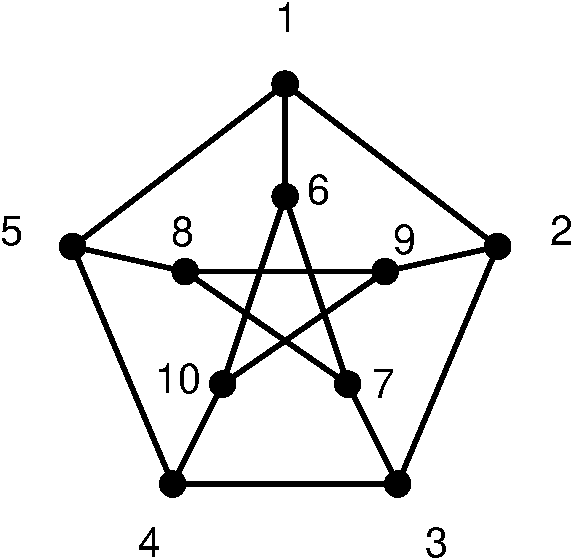
\includegraphics[width=1.5in,clip]{G1}}
        \hspace{17mm}
        \subfigure[$G_2$]{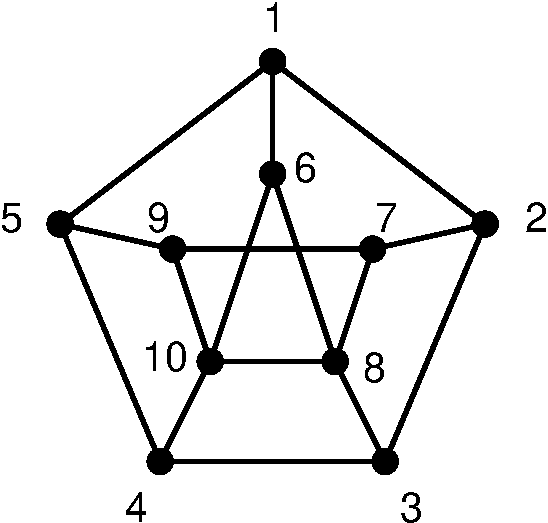
\includegraphics[width=1.5in,clip]{G4}} }
\mbox{  \subfigure[$G_3$]{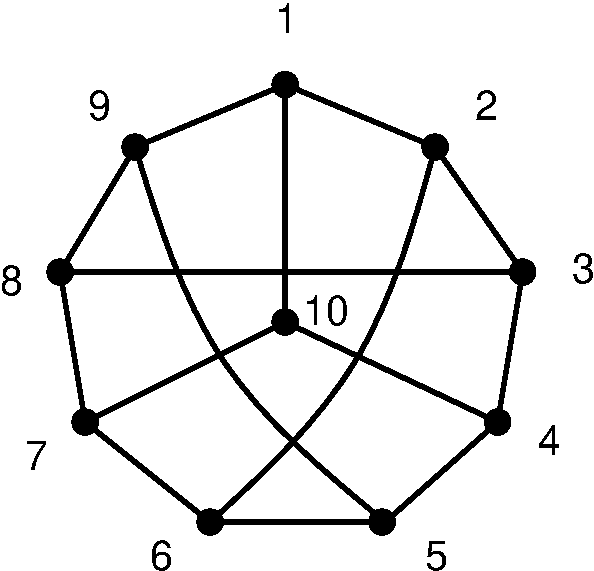
\includegraphics[width=1.5in,clip]{G2}}
        \hspace{17mm}
        \subfigure[$G_4$]{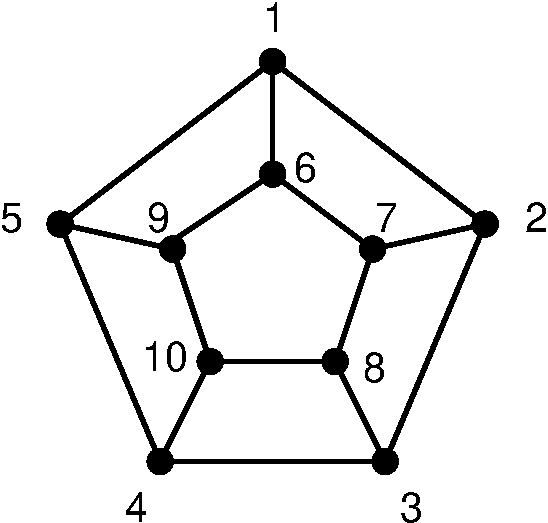
\includegraphics[width=1.5in,clip]{G3}}
        }
\end{center}
\caption{Which graphs are isomorphic?}
\label{fig:isog}
\end{figure}

\iffalse

\begin{figure}[h] %[htbp]
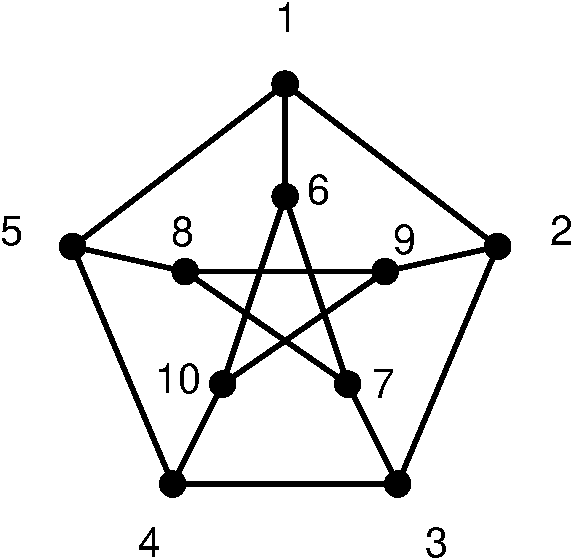
\includegraphics[width=1.5in,clip]{G1}
\caption{$G_1$}
\label{fig:G1}
\end{figure}

\begin{figure}[h] %[htbp]
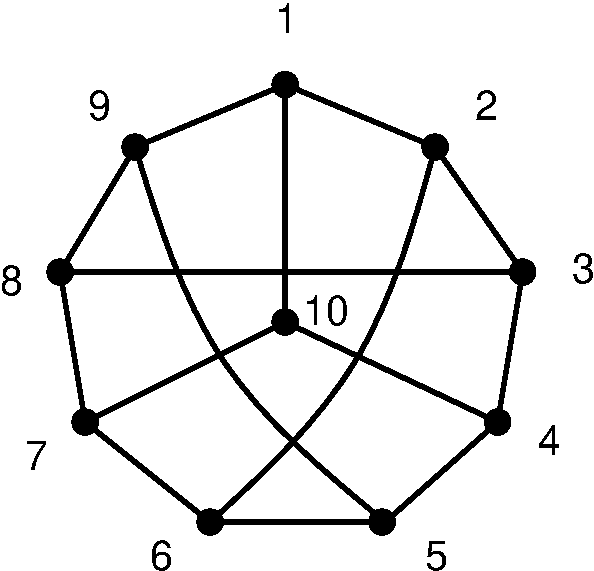
\includegraphics[width=1.5in,clip]{G2}
\caption{$G_2$}
\label{fig:G2}
\end{figure}

\begin{figure}[h] %[htbp]
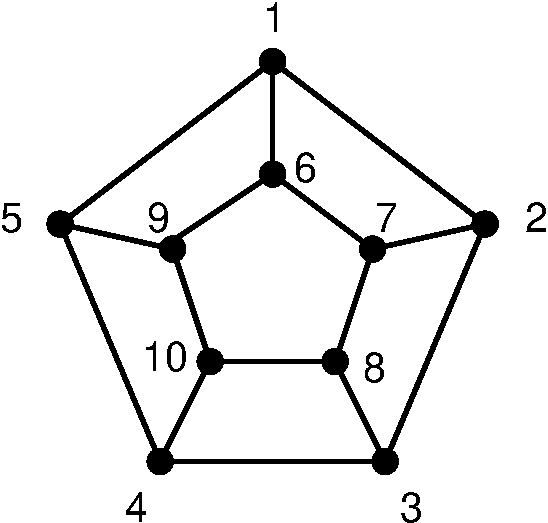
\includegraphics[width=1.5in,clip]{G3}
\caption{$G_3$}
\label{fig:G3}
\end{figure}

\begin{figure}[h] %[htbp]
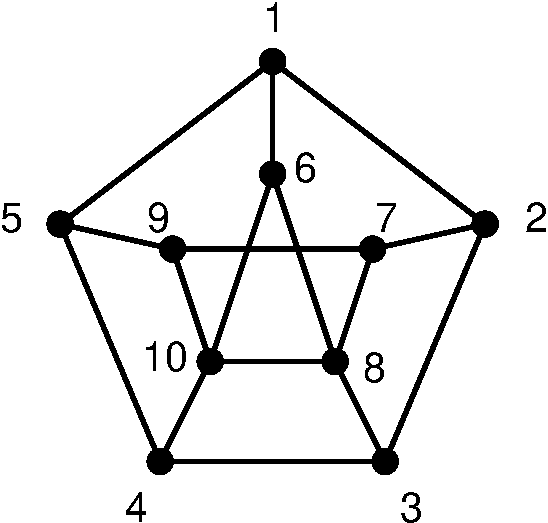
\includegraphics[width=1.5in,clip]{G4}
\caption{$G_4$}
\label{fig:G4}
\end{figure}
\fi
\rubric{
[1pt] $G_1$ and $G_3$ are isomorphic. \par
[2pts] Correct isomorphism. \par
[1pt] $G_2$ is not isomorphic to $G_1$ or $G_4$.\par
[1pt] Correct justification for why $G_2$ is not isomorphic to $G_1$ or $G_4$. \par
[1pt] $G_4$ is not isomorphic to $G_1$ or $G_2$. \par
[1pt] Correct justification for why $G_4$ is not isomorphic to $G_1$ or $G_2$. \par
[3pts] Proof for one of the property on why it is preserved under isomorphism. (See (a)).
}
\solution{
$G_1$ and $G_3$ are isomorphic.  In particular, the function
$f:V_1 \to V_3$ is an isomomorphism, where
\begin{align*}
&f(1)=1 \quad&& f(2)=2 \quad&& f(3)=3 \quad&& f(4)=8 \quad&& f(5)=9 \\
&f(6)=10 \quad&& f(7)=4 \quad&& f(8)=5 \quad&& f(9)=6 \quad&& f(10)=7
\end{align*}

$G_1$ and $G_4$ are not isomorphic to $G_2$: $G_2$ has a vertex of degree
four and neither $G_1$ nor $G_4$ has one.

$G_1$ and $G_4$ are not isomorphic: $G_4$ has a simple cycle of length
four and $G_1$ does not.

}

\eparts
\end{problem}


\begin{problem}{20}
%TODO: can change the actual graph (but still keep the 4-clique so that 4 colors are necessary)
6.042 is often taught using recitations.  Suppose it
happened that 8 recitations were needed, with two or three staff members
running each recitation.  The assignment of staff to recitation sections
is as follows:

\begin{itemize}
\item R1:  \TAonename, \TAtwoname, \TAthreename 
\item R2:  \TAonename, \TAeightname, \TAninename
\item R3:  \TAtwoname, \TAfivename
\item R4:  \TAsixname, \TAeightname, \TAsevenname
\item R5:  \TAsixname, \TAfourname, \TAninename
\item R6:  \TAfourname, \TAfivename
\item R7:  \TAfourname, \TAeightname
\item R8:  \TAtwoname, \TAfivename, \TAninename 
\end{itemize}

Two recitations can not be held in the same 90-minute time slot if some
staff member is assigned to both recitations.  The problem is to determine
the minimum number of time slots required to complete all the recitations.

\bparts

\ppart{10} Recast this problem as a question about coloring the
vertices of a particular graph.  Draw the graph and explain what the
vertices, edges, and colors represent.
\rubric{
[2pts] Vertex is a recitation section.\par
[2pts] Edge connects recitations that cannot be scheduled at same time.\par
[2pts] Color corresponds to time slot.\par
[3pts] Correctly drawn graph.
}
\solution{
    Each vertex in the graph below represents a recitation
section.  An edge connects two vertices if the corresponding
recitation sections share a staff member and thus can not be scheduled
at the same time.  The color of a vertex indicates the time slot of
the corresponding recitation.

\begin{center}
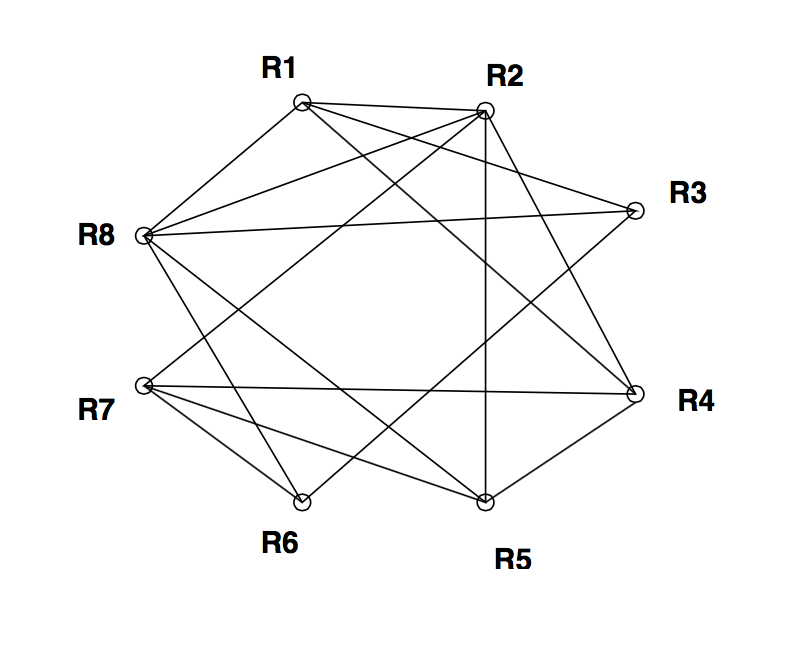
\includegraphics[height=2in]{sol_a.png}
\end{center}
}

\ppart{10}
Show a coloring of this graph using the fewest possible
colors.  What schedule of recitations does this imply?
\rubric{
[7pts] Any valid grouping of recitations. (Should be right if the number of time slots is)\par
[3pts] 4 time slots because 4 colors.
}
\solution{
Four colors are necessary and sufficient. To see why they
are \emph{sufficient}, consider the coloring:
\begin{center}
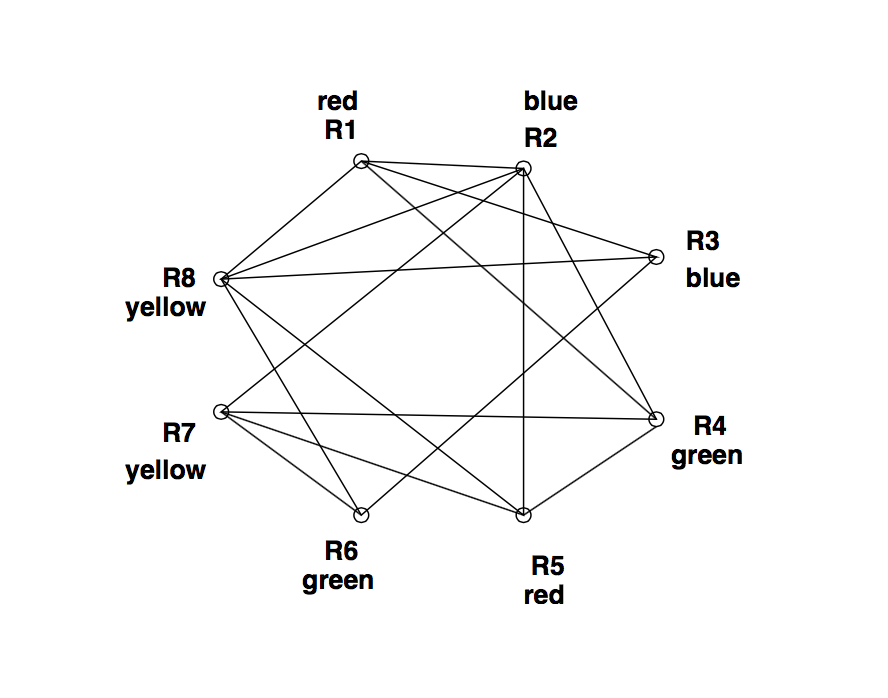
\includegraphics[height=2in]{sol_b.png}
\end{center}
This corresponds to the following assignment of recitations to four
time slots:
\begin{enumerate}

\item R1, R5

\item R2, R3

\item R4, R6

\item R7, R8

\end{enumerate}
Other schedules are also possible.

To see why 4 colors are \emph{necessary}, look at the subgraph defined
by the vertices for R2, R4, R5, and R7.  This is the complete graph on 4
vertices, and it obviously needs 4 colors.
}

\eparts

\end{problem}

% Problem
\begin{problem}{20}
Suppose you have a graph as shown below. Every node on the left is adjacent 
to every node on the right except the node directly across from it.
\begin{center}
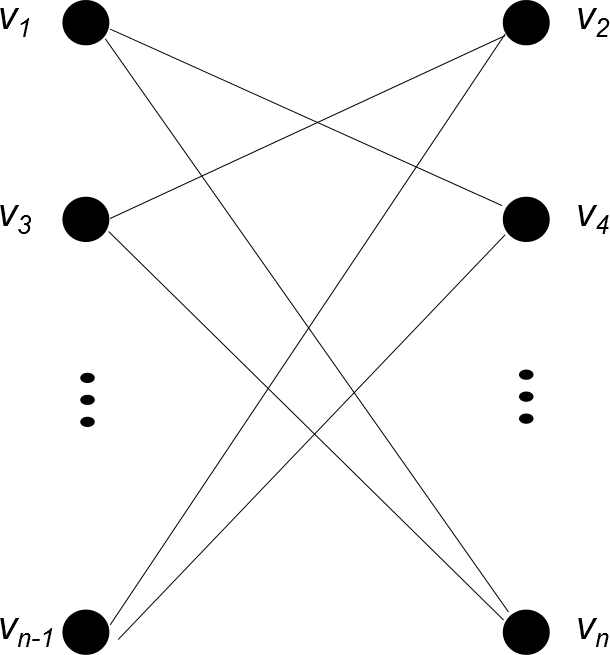
\includegraphics[height = 2in]{coloring}
\end{center}

\bparts

% part a
\ppart{5}
Find the chromatic number of the graph.
\rubric{
[5pts] 2 colors.
}
% part a solution
\solution{
We can color each node on the left side with red and each node on the right 
with blue since no edges form between nodes on the same side. Thus, the 
chromatic number is 2.
}

% part b
\ppart{5}
The graph pictured above is often referred to as \textit{bipartite}.

\begin{definition*}
A graph $G = (V,E)$ is \underline{bipartite} if the set of vertices, $V$, can 
be split into two subsets $V_l$ and $V_r$ such that all edges in $G$ connect 
nodes in $V_l$ to nodes in $V_r$. 
\end{definition*}

Now recall from lecture the Greedy Coloring Algorithm: \\
\textbf{Greedy Coloring Algorithm:} For a graph $G = (V,E)$ and an ordering 
of vertices $v_1, v_2, \cdots, v_n$
\begin{enumerate}
\item Color $v_1$ with a new color $c_1$.
\item For each vertex $v_i$, if $v_i$ shares an edge with with any earlier vertex,
    $v_j$, colored $c_k$, then it cannot be colored $c_k$. Choose the lowest available
    color for $v_i$.
\end{enumerate}

Find an ordering of the vertices $\{v_1, v_2, \cdots, v_n\}$ such that the 
Greedy Coloring Algorithm uses exactly 2 colors.
% part b solution
\rubric{
[5pts] $v_1, v_3, v_5, \cdots v_{n-1}, \cdots, v_2, v_4, \cdots, v_n$
}
\solution{
Since none of the vertices on the left share an edge, we can color all of 
them with the same color, so we iterate through all the left nodes, then all 
the right nodes with the ordering, $v_1, v_3, v_5, \cdots v_{n-1}, \cdots, v_2, v_4, \cdots, v_n$. 
The left side uses only one color and the right side uses only one color 
similar to the solution in part (a).
}

% part c
\ppart{5}
Find an ordering such that the Greedy Coloring Algorithm uses exactly $n/2$ colors.
% part c solution
\rubric{
[5pts] Alternating sides
}
\solution{
Notice that alternating across left and right with the greedy algorithm forces us to pick a new color 
every time we are on the left side. Thus, we can choose the ordering $v_1, v_2, \cdots 
v_{n/2}, \cdots v_n$ to get $n/2$ colors.
}

% part d
\ppart{5}
Prove your answer in part (c) by induction for all even integers $n$.
% part d solution
\proofrubric[Not a proof by induction]{
[1pt] Induction hypothesis\par
[1pt] Base case\par
[1pt] Show $P(n)$ implies $P(n+2)$\par
[2pts] Corrective inductive step
}{0}
\solution{
\begin{proof}
$P(n)$ is defined to be: For a bipartite graph with $n$ vertices (labeled in 
the pattern as shown in the graph), with edges as shown in the graph, 
applying the Greedy Coloring Algorithm to the vertex ordering $v_1, v_2 \cdots
 v_n$ uses exactly $n/2$ colors for all even integers $n$. In addition, the coloring consists of the first $n/2$ colors on each side across from one another.

{ \bf Base Case } (n = 2) There are no edges in this case, so the Greedy 
Coloring Algorithm uses only one color.

{ \bf Inductive Step }
Assume that $P(n)$ is true. We will 
show that this implies $P(n+2)$. Denote our two new nodes $v_{n+1}$ and $v_{n+2
}$. $v_{n+1}$ is connected to $\{v_2, v_4, \cdots v_n\}$ and $v_{n+2}$ is 
connected to $\{v_1, v_3,  \cdots v_{n-1} \}$. Since by $P(n)$, $v_{n+1}$ is 
connected to $n/2$ different colors, the Greedy Coloring Algorithm will 
choose a different color $c_{n/2 + 1}$. For $v_{n+2}$,  the Greedy Algorithm 
will color it $c_{n/2 + 1}$ since its connected to $v_1, v_3, \cdots v_{n-1}$ 
which are the first $n/2$ colors. Thus, the new nodes are both a new color.\\

Thus, by induction, $P(n+2)$ is true.

\end{proof}
}
\eparts

\end{problem}




\end{document}
